\chapter{Introduction} \label{chap:intr}
%
%
From the middle of the 20th century onwards, a scientific domain has gained in interest: \acrfull{ai} \cite{russell_artificial_2009}. \acrshort{ai} is an \textquote{umbrella term} that includes multiple approaches and that envelops a large diversity of fields such as computer vision, natural language processing, voice recognition, etc.
An interesting approach of \acrshort{ai} is the ability of a machine to learn automatically. This field is called \acrfull{ml} and it has revolutionized several technology realms \cite{alom_history_2018}.
\textcite{mitchell_machine_1997} gives us a definition of what \acrshort{ml} is: \textquote{\textit{The concept of \acrshort{ml} relates to the question of how to construct computer programs that automatically improve with experience}}.

\textcite{arnold_introduction_2011} reported that one of the challenge of traditional machine learning, given a task of interest, is the selection of the most relevant features. While \acrshort{ml} uses handmade features, automatic learning of them using \acrfull{nn} can be used to tackle this issue. \acrfull{dl} architectures are based on this idea, composed of layers of non-linear processing. Since the previous decade, \acrshort{dl} has made breakthroughs and its fields of application have multiplied \cite{wason_deep_2018}. The accuracy of the models using this paradigm has also increased. For example, in 2015, the models submitted for the image classification task achieved on average 94.5\% of accuracy \cite{russakovsky_imagenet_2015}.

A type of \acrshort{dl} model, \acrfull{cnn}, has demonstrated its interest in applications such as image and speech processing, thanks to their high performance \cite{shawahna_fpga-based_2019}. However, the drive for improving the accuracy of such models is to increase their size, which comes at the price of a large computational and memory cost (billions of operations and millions of parameters) \cite{szegedy_going_2014, khan_survey_2020}. For example, ResNet \cite{he_deep_2015} requires 25.6M parameters and 11.3B floating point operations for $224 \times 224$ input images.

To implement and train such computationally-intensive models, dedicated accelerators seem to be be more suitable than general \acrfull{cpu} \cite{liu_fpga-based_2019}. \acrfull{gpu}, \acrfull{asic} and \acrfull{fpga} can, therefore, be used to improve the throughput and latency of the \acrshort{cnn}. The dominant platforms to perform \acrshort{cnn} inferences are \acrshort{cpu} and \acrshort{gpu} clusters because they offer the best performance in terms of computational throughput but those are power-hungry \cite{liu_uniform_2019}.

\acrshort{fpga} and \acrshort{asic} seem then to be a promising solution because they are more energy-efficient. This has been demonstrated by \textcite{qasaimeh_comparing_2019}, where FPGA outperforms \acrshort{gpu} as the vision application’s pipeline complexity grows (which is the case for \acrshort{cnn}). We can observe in Table \ref{tab:benchener} the FPGA’s energy reduction ratios with respect to GPU for various vision application’s pipeline. Moreover, an \acrshort{fpga}-based \acrshort{cnn} accelerator is more suitable than an \acrshort{asic} because it is more time and cost-effective when designing and verifying a process \cite{motamedi_placid_2017}.
%
\begin{table}
    \center
    \begin{tabular}{|c|c|}
        \hline
        Pipeline & Energy/frame (mJ/f) \\
        \hline
        Background Subtraction & 1.74 $\times$\\
        \hline
        Color Segmentation & 1.86 $\times$ \\
        \hline
        Harris Corners Tracking & 3.94 $\times$ \\
        \hline
        Stereo Block Matching & 8.83 $\times$ \\
        \hline
    \end{tabular}
    \caption{FPGA’s Reduction Ratios with respect to GPU \cite{qasaimeh_comparing_2019}}
    \label{tab:benchener}
\end{table}

Still, while \acrshort{gpu} is currently the most dominant platform to perform \acrshort{cnn}s, trends confirm that \acrshort{fpga} will be more suitable to accelerate \acrshort{cnn}s. Two reasons can explain that: first, the advances in \acrshort{fpga} technology show that the performance disparity between \acrshort{fpga} and \acrshort{gpu} has lessened; second, recent trends in \acrshort{cnn} utilize sparsity and extreme compact data types which is in the favor of the \acrshort{fpga}s, because they are designed to handle irregular parallelism and custom data type \cite{nurvitadhi_can_2017}. However, \acrshort{fpga} is resource-constraint (limited memory, I/O bandwidth, and computing resources) and the challenge is to find a mapping between the computational model and the execution model.

\acrshort{cnn} consists of two phases: a training stage where the model learns (back-propagation algorithm \cite{lecun_backpropagation_1989}) and the inference stage where the model makes a prediction on new data samples (feed-forward algorithm \cite{zhang_optimizing_2015}). We can see the process in Figure \ref{fig:traininf}. Usually, \acrshort{cnn}s are trained once using \acrshort{gpu} or \acrshort{fpga} and inference is executed every time the \acrshort{cnn} has a new input to process. Most efforts have then been focused on accelerating the inference stage. The core of this work is therefore aimed at proposing a way to accelerate the inference of a model on \acrshort{fpga}.
%
\begin{figure}
    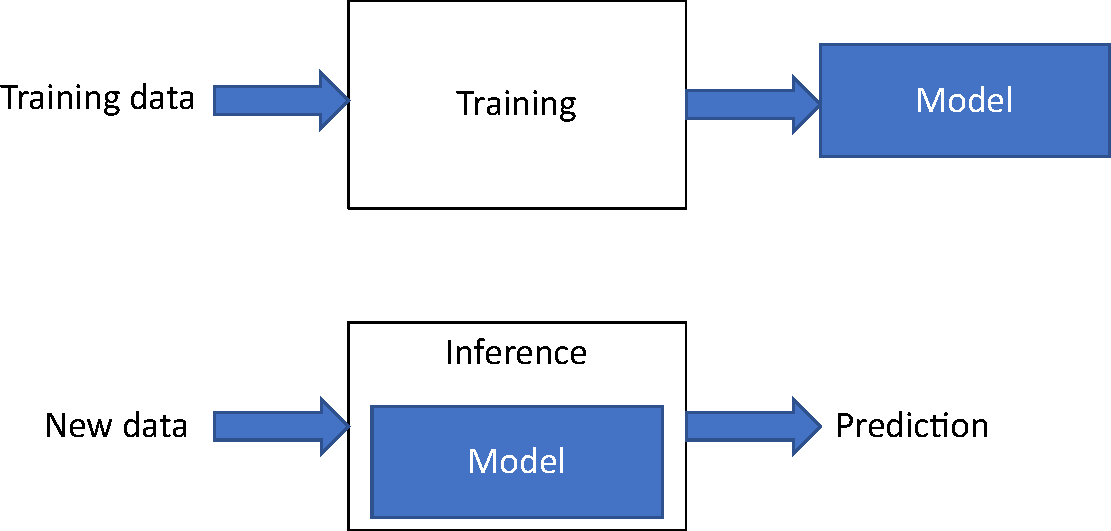
\includegraphics[width=\textwidth]{traininf.pdf}
    \caption{\acrshort{cnn} setup for predicting new data}
    \label{fig:traininf}
\end{figure}

The inference can be accelerated using various optimizations can be grouped into 3 main categories, according to \textcite{abdelouahab_accelerating_2018}:
\begin{itemize}
    \item \textbf{Algorithmic Optimizations}: the computational cost of the convolution can be reduced by vectorizing the operation or using faster algorithms.
    \item \textbf{Datapath Optimization}: because of the limited resources on an FPGA, memory is often the bottleneck and optimizing the memory management can increase the throughput.
    \item \textbf{\acrshort{cnn} model Optimization}: an important issue of \acrshort{cnn} is their computational complexity and hardware utilization. A solution is then to use approximate computing to trade accuracy for acceleration. This kind of optimization is going to be the key point of this work because the \acrshort{cnn} size and arithmetic complexity are the major issues when implementing a \acrshort{cnn} on \acrshort{fpga}.
\end{itemize}

This work focus on weights pruning because it is not efficiently exploitable on a \acrshort{gpu}. The irregular data access and the custom data type of the non-pruned weights show it is more suitable to implement pruning on \acrshort{fpga} rather than \acrshort{gpu}. Therefore, this work concentrates on building an architecture using pruning on depthwise separable convolution, an alternative way to perform convolution which uses fewer parameters and has a lesser computational complexity. The objective of this work is then to build an efficient architecture on \acrshort{fpga} implementing a sparse \acrshort{cnn} network using depthwise separable convolution. To show the achievability, we have chosen MobileNetV2 because it offers state-of-the-art performance.

<Insert principal results>
%
%
\section*{Structure of the thesis}
%
%
This master thesis is composed of 7 chapters.

Chapter \ref{chap:cnn} details the theory behind \acrshort{cnn} and goes deeper into its computational background. We also explore algorithmic and model optimizations to reduce the cost of the convolution operation and the size of the models.

The concept of \acrshort{fpga} is explained in Chapter \ref{chap:fpga}. We detail there the workflow and \acrshort{fpga} designs. The chapter also details datapath optimizations which reduce the inefficiency of the convolution on \acrshort{fpga}.

Using knowledge of Chapters \ref{chap:cnn} and \ref{chap:fpga}, we explain in chapter \ref{chap:inf} what is the focus of this work, pruning. We detail our hypothesis and \acrshort{fpga} architectures that have managed pruning schemes.

Chapter \ref{chap:arch} explains on how to build an efficient architecture on \acrshort{fpga} and uses this knowledge to design our architecture using pruning and depthwise separable convolution.

Chapter \ref{chap:measure} explains the simulation on SystemVerilog of the architecture developed in Chapter \ref{chap:arch} and details the experiments on this simulation. Potential improvements will be discussed.

Finally, a conclusion on results obtained and discussion on future works is done in Chapter \ref{chap:ccl}.

\afterpage{\blankpage}
\cleardoublepage
\newpage
